\documentclass[11pt]{article}

\usepackage[margin=1in]{geometry}
\usepackage[T1]{fontenc}
\usepackage{lmodern}
\usepackage{microtype}
\usepackage{amsmath,amssymb,amsthm}
\usepackage{booktabs}
\usepackage{graphicx}
\usepackage{caption}
\usepackage{subcaption}
\usepackage{xcolor}
\usepackage[numbers,sort&compress]{natbib}
\usepackage[hidelinks]{hyperref}
\usepackage{enumitem}

\graphicspath{{../figures/}}
\newcommand{\accMnistMlpRelu}{97.57}
\newcommand{\accMnistMlpGelu}{97.91}
\newcommand{\accMnistMlpHelu}{91.50}
\newcommand{\accMnistMlpIdentity}{91.50}
\newcommand{\accFashionMlpRelu}{88.14}
\newcommand{\accFashionMlpGelu}{88.16}
\newcommand{\accFashionMlpHelu}{83.33}
\newcommand{\accFashionMlpIdentity}{83.33}
\newcommand{\accFashionCnnRelu}{91.48}
\newcommand{\accFashionCnnGelu}{91.96}
\newcommand{\accFashionCnnHelu}{90.35}
\newcommand{\accFashionCnnIdentity}{90.32}
\newcommand{\rTwoHelu}{1.00000}
\newcommand{\rTwoRelu}{0.957}
\newcommand{\notchHelu}{2.81}
\newcommand{\accMoonsRelu}{98.7}
\newcommand{\accMoonsGelu}{98.4}
\newcommand{\accMoonsHelu}{88.0}
\newcommand{\accMoonsIdentity}{87.7}
\newcommand{\accSpiralsRelu}{99.6}
\newcommand{\accSpiralsGelu}{99.6}
\newcommand{\accSpiralsHelu}{63.0}
\newcommand{\accSpiralsIdentity}{64.9}

\IfFileExists{generated/macros_variants.tex}{\newcommand{\bestVariantFashion}{$[0.5,\infty]\times0.2$}
\newcommand{\bestVariantFashionAcc}{86.36}
\newcommand{\bestVariantSpirals}{$[0.5,\infty]\times0.2$}
\newcommand{\bestVariantSpiralsAcc}{98.3}
}{}
\IfFileExists{generated/macros_sawtooth.tex}{\newcommand{\accSawFashion}{10.1}
\newcommand{\accSawMoons}{50.2}
\newcommand{\accSawSpirals}{54.6}
\newcommand{\mseSawSin}{0.49}
\newcommand{\rTwoSaw}{0.39}
\newcommand{\sawBestMoons}{71}
\newcommand{\sawBestMoonsLr}{10^{-5}}
\newcommand{\sawDriftDefault}{257}
\newcommand{\sawDescentLow}{84}
}{}
\IfFileExists{generated/macros_stepslope.tex}{\newcommand{\accSsSmallFashion}{82.6}
\newcommand{\accSsSmallSpirals}{64.2}
\newcommand{\accSsSmallMoons}{88.9}
\newcommand{\mseSsSmallSin}{0.403}
\newcommand{\rTwoSsSmall}{1.0000}
\newcommand{\accSsMidFashion}{84.6}
\newcommand{\accSsMidSpirals}{92.2}
\newcommand{\accSsMidMoons}{98.9}
\newcommand{\mseSsMidSin}{0.008}
\newcommand{\rTwoSsMid}{0.9770}
\newcommand{\accSsOneFashion}{86.2}
\newcommand{\accSsOneSpirals}{99.5}
\newcommand{\accSsOneMoons}{98.7}
\newcommand{\mseSsOneSin}{0.001}
\newcommand{\rTwoSsOne}{0.9120}
\newcommand{\accSsFineFashion}{86.6}
\newcommand{\accSsFineSpirals}{86.4}
\newcommand{\accSsFineMoons}{98.4}
\newcommand{\mseSsFineSin}{0.305}
\newcommand{\rTwoSsFine}{0.9192}
}{}
\IfFileExists{generated/macros_stepslope_tune.tex}{\newcommand{\ssBestW}{2}
\newcommand{\ssBestDelta}{1}
\newcommand{\ssBestVal}{87.41}
\newcommand{\geluVal}{87.28}
\newcommand{\reluVal}{86.97}
\newcommand{\finalMnistRelu}{97.57}
\newcommand{\finalMnistGelu}{97.91}
\newcommand{\finalMnistSs}{97.09}
\newcommand{\finalMnistPGelu}{0.0107}
\newcommand{\finalFashionRelu}{88.14}
\newcommand{\finalFashionGelu}{88.16}
\newcommand{\finalFashionSs}{87.56}
\newcommand{\finalFashionPGelu}{0.0359}
\newcommand{\finalCnnRelu}{91.48}
\newcommand{\finalCnnGelu}{91.96}
\newcommand{\finalCnnSs}{91.95}
\newcommand{\finalCnnPGelu}{0.977}
\newcommand{\depthGeluOne}{87.03}
\newcommand{\depthSsOne}{86.67}
\newcommand{\depthGeluTwo}{87.03}
\newcommand{\depthSsTwo}{87.20}
\newcommand{\depthGeluFour}{86.53}
\newcommand{\depthSsFour}{78.88}
\newcommand{\depthGeluEight}{86.17}
\newcommand{\depthSsEight}{13.21}
}{}

\newtheorem{proposition}{Proposition}
\newcommand{\helu}{\mathrm{HeLU}}
\newcommand{\R}{\mathbb{R}}

\title{Does a Notch Make a Non-Linearity?\\
\large An Empirical Evaluation of HeLU against ReLU and GELU}
\author{HeLU activation study\\
\small \texttt{helu-activation-research/} in \texttt{lukeabraham24777/unblock-me-game}}
\date{September 2026}

\begin{document}
\maketitle

\begin{abstract}
We evaluate a proposed activation function, HeLU, defined as $\helu(x)=x$ everywhere except on the
interval $0.5\le x\le 0.6$, where $\helu(x)=0.9x$. The hypothesis under test is that networks trained
with HeLU outperform networks trained with ReLU or GELU. We compare the three activations, plus an
identity (purely linear) control, under identical architectures, optimisers, and seeds on one-dimensional
function regression, two-dimensional non-linearly separable classification, MNIST and Fashion-MNIST
with multilayer perceptrons, Fashion-MNIST with a small convolutional network, a depth sweep, and a
mechanistic analysis of the trained networks. \textbf{The hypothesis is not supported.} On every task
whose solution requires a non-linear decision function, HeLU networks perform substantially and
statistically significantly worse than ReLU and GELU networks, and are statistically indistinguishable
from the linear control. A least-squares linear fit explains a fraction \rTwoHelu{} of the variance of
a trained HeLU network's outputs (versus \rTwoRelu{} for ReLU), and only \notchHelu\% of hidden
pre-activations fall inside the notch after training. HeLU is therefore best understood as an
approximately linear map with a small, rarely visited perturbation, and it inherits the expressivity
limits of deep linear networks. The one setting in which HeLU comes within a point of ReLU and GELU is
the convolutional network, where max-pooling supplies the non-linearity that the activation does not,
and the linear control comes equally close there. An ablation over sixteen variants of the notch
(moved, deepened, or widened) shows that the deficit is a property of the notch design rather than of
its particular constants, and a periodic sawtooth function, tested as a further alternative, fails
differently again: it is expressive but its constant slope makes the gradient blind to which period a
unit is in, and training never leaves chance. A final continuous design whose slope steps up by
$\delta$ per unit segment works only when $\delta$ is large enough to make the network visibly
non-linear; at the proposed $\delta=0.01$ it is the identity in all but name. Tuned on a validation
split, it ties GELU on a convolutional network and trails it by under a point on the MLPs, but its
unbounded slope makes it collapse to chance at eight hidden layers. All code, raw results, and figures
are released alongside this document.
\end{abstract}

\section{Introduction}

The choice of activation function sets the family of functions a neural network can represent and shapes
the optimisation landscape. ReLU~\citep{nair2010relu} and GELU~\citep{hendrycks2016gelu} dominate current
practice; the former is cheap and sparse, the latter is smooth and has become the default in transformer
architectures. Proposals for new activations are common, and the standard of evidence is empirical: a new
function is judged by whether models trained with it reach better accuracy or lower loss than the same
models trained with the incumbents~\citep{ramachandran2018swish}.

This report applies that standard to a proposed activation, which we refer to as HeLU. It is defined as
\begin{equation}
  \helu(x) \;=\;
  \begin{cases}
    0.9\,x & \text{if } 0.5 \le x \le 0.6,\\
    x      & \text{otherwise.}
  \end{cases}
  \label{eq:helu}
\end{equation}
The claim we set out to verify is that HeLU is \emph{superior} to ReLU and GELU, i.e.\ that networks
trained with HeLU achieve better held-out performance under matched conditions. We fixed the
following reading of the outcome before running the full experimental sweep: the hypothesis is supported if HeLU
attains higher mean test accuracy (or lower test error) than both ReLU and GELU on the majority of tasks,
with the difference significant at $p<0.05$ under Welch's $t$-test~\citep{welch1947} across seeds.

\paragraph{Contributions.}
\begin{enumerate}[nosep]
  \item A controlled comparison of HeLU, ReLU, and GELU, plus an identity control, over eight experiments
        spanning regression, classification, image benchmarks, and depth (Section~\ref{sec:setup}).
  \item A negative result: HeLU is statistically indistinguishable from a linear network on every task
        we tried and significantly worse than ReLU and GELU whenever the task is non-linear
        (Section~\ref{sec:results}).
  \item A mechanistic explanation. The notch is visited by roughly \notchHelu\% of pre-activations, and
        a linear model fits the trained HeLU network almost perfectly (Section~\ref{sec:mechanism}).
\end{enumerate}

\section{The HeLU function}
\label{sec:helu}

Figure~\ref{fig:activation} plots the three activations and their derivatives. Several properties of
\eqref{eq:helu} follow directly from the definition.

\begin{figure}[t]
  \centering
  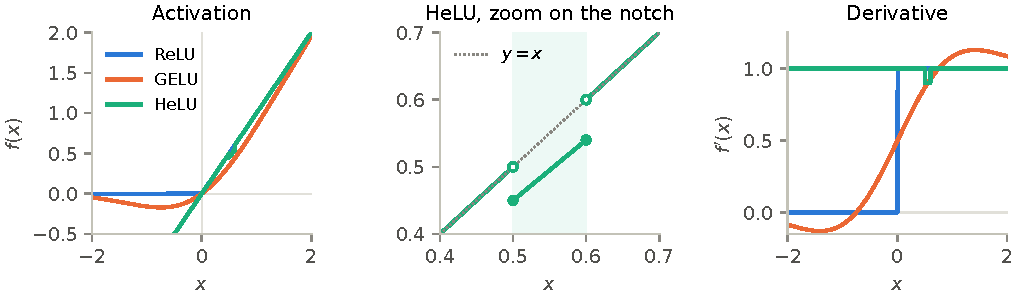
\includegraphics[width=\linewidth]{fig_activation.pdf}
  \caption{Left: ReLU, GELU, and HeLU on $[-2,2]$. Centre: HeLU near the notch; filled and open circles
  mark the value taken and not taken at each edge. Right: derivatives. HeLU's derivative is 1 except
  on $[0.5,0.6]$, where it is $0.9$.}
  \label{fig:activation}
\end{figure}

\begin{itemize}[nosep]
  \item \textbf{It is almost the identity.} $|\helu(x)-x|=0.1|x|\le 0.06$, and this deviation is
        non-zero only on an interval of width $0.1$.
  \item \textbf{It is discontinuous.} At $x=0.5$ the function jumps from $0.5$ to $0.45$; at $x=0.6$ it
        jumps from $0.54$ to $0.6$. Neither ReLU nor GELU has a discontinuity.
  \item \textbf{Its derivative is nearly constant.} $\helu'(x)=1$ outside the notch and $0.9$ inside;
        automatic differentiation reproduces exactly this (Figure~\ref{fig:activation}, right). Gradients
        therefore flow through HeLU layers essentially unchanged, as in a linear network.
  \item \textbf{It is non-polynomial.} By the theorem of \citet{leshno1993multilayer}, a
        single-hidden-layer network with HeLU activations is a universal approximator in the limit of
        infinite width. The theorem, however, says nothing about how many units, how large the weights,
        or how difficult the optimisation problem must be. For HeLU the non-linear budget of each unit is
        a perturbation of amplitude at most $0.06$ confined to a band of width $0.1$, so expressing a
        non-linear function of order-one amplitude requires either very many units whose
        pre-activations land in the notch or very large output weights.
\end{itemize}

\noindent
The natural null model for HeLU is therefore a \emph{deep linear network}, whose behaviour is well
understood~\citep{saxe2014exact}: regardless of depth or width it can only represent a single affine map
of its input. We include the identity activation as an explicit control so that this null can be tested
directly rather than assumed.

\section{Experimental setup}
\label{sec:setup}

All experiments use PyTorch~\citep{paszke2019pytorch} on CPU with the Adam
optimiser~\citep{kingma2015adam}. Within each experiment the architecture, learning rate, batch size,
number of steps or epochs, data ordering, and parameter-initialisation seed are identical across
activations; the activation module is the only thing that changes. Hyper-parameters were fixed in
advance to common defaults and were not tuned per activation. Results are reported as mean $\pm$
sample standard deviation across seeds, and differences involving HeLU are tested with Welch's
unequal-variance $t$-test.

\begin{description}[nosep,leftmargin=1.5em]
  \item[E1: Function shape.] Analytic evaluation of $f$ and $f'$ (Figure~\ref{fig:activation}).
  \item[E2: 1-D regression.] An MLP with two hidden layers of 64 units maps $x\in[-2,2]$ to one of
        four targets: $\sin 3x$, $|x|$, $x^2$, and the step $\mathbf 1[x>0]$. Training uses 512 points
        with Gaussian noise ($\sigma=0.05$), 3000 full-batch Adam steps at learning rate $3\times10^{-3}$;
        the test MSE is computed on 2000 noise-free points. 5 seeds.
  \item[E3: 2-D classification.] Two-moons and two-spirals datasets (600 training points, 4000 test
        points), same MLP with a two-way softmax output, 3000 steps. 5 seeds.
  \item[E4: MNIST and Fashion-MNIST, MLP.] $784\!-\!256\!-\!256\!-\!10$ MLP, batch size 128, learning
        rate $10^{-3}$, 5 epochs. 5 seeds each~\citep{lecun1998mnist,xiao2017fashion}.
  \item[E5: Fashion-MNIST, CNN.] Two $3\times3$ convolutions (32 and 64 channels), each followed by the
        activation and $2\times2$ max-pooling, then a 128-unit fully connected layer with the activation
        and a linear classifier. Same optimiser settings, 5 epochs, 3 seeds.
  \item[E6: Depth sweep.] Fashion-MNIST MLP with 128-unit hidden layers and 1, 2, 4, or 8 hidden
        layers, 3 epochs, 3 seeds.
  \item[E7: Linearity and notch occupancy.] For the Fashion-MNIST MLP we measure (i) the $R^2$ of the
        best least-squares affine map from the 784-dimensional input to the network's 10 logits, computed
        on 2000 test images, and (ii) the fraction of hidden pre-activations lying in $[0.5,0.6]$, both at
        initialisation and after 3 epochs of training. 3 seeds.
  \item[E8: Kernel cost.] Wall time of forward plus backward through the activation alone on a
        $4\times10^6$-element tensor, 20 repetitions.
  \item[E9: Notch variants.] Sixteen variants of \eqref{eq:helu} obtained by moving the notch
        ($[0.5,0.6]$, $[0.1,0.2]$, $[-0.05,0.05]$), deepening it (scale $0.9$, $0.8$, $0.5$, $0.2$),
        widening it ($[0.5,1.0]$, $[0.5,2.0]$, $[0.5,\infty)$ at scale $0.2$), or replacing it with a
        wide symmetric band around zero ($[-0.68,0.68]$ at scale $0.5$). Each variant is run under
        the E2 protocol on $\sin 3x$ and $x^2$, the E3 protocol on moons and spirals, and the E4
        Fashion-MNIST MLP protocol for 3 epochs, all with 3 seeds.
  \item[E10: Sawtooth function.] The function that, on each interval $[k,k+2)$ for $k\in 2\mathbb Z$,
        rises linearly from $(k,0)$ to $(k+2,1)$, i.e.\ $T(x)=x/2-\lfloor x/2\rfloor$. It is run under the
        E9 protocol, and we additionally record the $R^2$ of a linear fit to the trained Fashion-MNIST
        network, a learning-rate sweep over $\{10^{-2},10^{-3},10^{-4},10^{-5}\}$ with the standard
        deviation of first-layer pre-activations before and after training, and a descent-direction test:
        on 50 mini-batches at initialisation, a plain gradient step of size $\eta$ is taken and we record
        whether the batch loss actually decreased.
  \item[E11: Slope-stepping function.] The continuous piecewise-linear function whose slope on segment
        $k=\lfloor x/W\rfloor$ is $1+\delta k$ for every integer $k$, so that the slope steps up by
        $\delta$ at each boundary. In closed form
        $P_{W,\delta}(x)=x+\delta\,[\,W k(k-1)/2 + k(x-kW)\,]$, a piecewise-linear approximation of
        $x+\delta x^2/(2W)$. Run under the E9 protocol for $(W,\delta)\in\{(1,0.01),(1,0.1),(1,1),(0.1,0.1)\}$,
        with the linear-fit $R^2$ of the trained Fashion-MNIST network.
  \item[E12: Tuned slope-stepping function versus GELU.] A grid over $W\in\{0.5,1,2\}$ and
        $\delta\in\{0.5,1,2,4\}$, each run for 3 epochs and 3 seeds on a 50k/10k train/validation split
        of the Fashion-MNIST training set, with GELU and ReLU run under the identical protocol as
        reference points. The setting with the best mean validation accuracy is then compared with GELU
        and ReLU under the full E4, E5, and E6 protocols (MNIST and Fashion-MNIST MLPs for 5 epochs and
        5 seeds, the Fashion-MNIST CNN for 5 epochs and 3 seeds, and the depth sweep), with Welch
        $t$-tests. The test sets are not used for selection.
\end{description}

\section{Results}
\label{sec:results}

\subsection{Function approximation}

\begin{figure}[t]
  \centering
  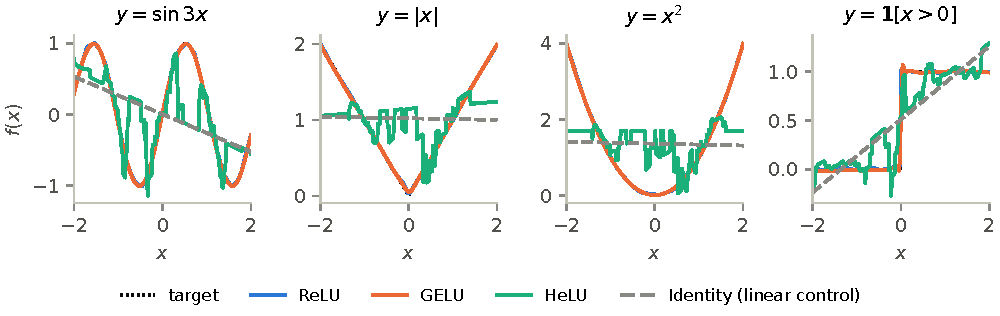
\includegraphics[width=\linewidth]{fig_reg1d_fits.pdf}\\[4pt]
  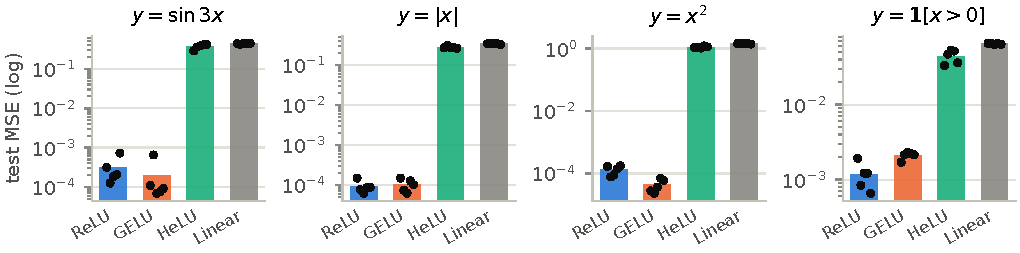
\includegraphics[width=\linewidth]{fig_reg1d_mse.pdf}
  \caption{1-D regression (E2). Top: the seed-0 fit of each network against the target (dotted).
  Bottom: test MSE on a log scale, bars are means over 5 seeds, dots are individual seeds. HeLU and the
  linear control coincide almost exactly.}
  \label{fig:reg1d}
\end{figure}

\begin{table}[t]
  \centering\small
  \caption{1-D regression test MSE (mean $\pm$ sd over 5 seeds). Lower is better.}
  \label{tab:reg1d}
  \begin{tabular}{lcccc}
\toprule
Target & ReLU & GELU & HeLU & Linear \\
\midrule
$sin(3x)$ & 0.0003 $\pm$ 0.0002 & 0.0002 $\pm$ 0.0003 & 0.3695 $\pm$ 0.0518 & 0.4364 $\pm$ 0.0093 \\
$|x|$ & 0.0001 $\pm$ 0.0000 & 0.0001 $\pm$ 0.0000 & 0.2792 $\pm$ 0.0193 & 0.3409 $\pm$ 0.0071 \\
$x^2$ & 0.0001 $\pm$ 0.0000 & 0.0000 $\pm$ 0.0000 & 1.1113 $\pm$ 0.0634 & 1.4361 $\pm$ 0.0297 \\
$\mathbf{1}[x>0]$ & 0.0012 $\pm$ 0.0005 & 0.0021 $\pm$ 0.0002 & 0.0443 $\pm$ 0.0092 & 0.0646 $\pm$ 0.0012 \\
\bottomrule
\end{tabular}

\end{table}

Figure~\ref{fig:reg1d} and Table~\ref{tab:reg1d} summarise E2. ReLU and GELU networks fit all four
targets closely, with test MSE of order $10^{-4}$ to $10^{-3}$. The HeLU network does \emph{not} collapse
to the linear control's straight line: with full-batch training on a one-dimensional input, gradient
descent does find the notch and uses it. What it builds with it, however, is a jagged staircase. Because
the only non-linear features of HeLU are its two jump discontinuities, the network can represent
vertical jumps but not smooth curvature, and the fit consists of a linear trend decorated with
irregular steps of amplitude comparable to the notch itself. The resulting test MSE is three orders of
magnitude worse than ReLU or GELU on $\sin 3x$, $|x|$, and $x^2$ (Table~\ref{tab:reg1d}), and only
$15$--$25\%$ better than the linear control. The step target is the most favourable case for HeLU, since
a discontinuity is exactly what it can express, and even there its error is $30$--$40\times$ that of
ReLU and GELU.

\subsection{Non-linearly separable classification}

\begin{figure}[t]
  \centering
  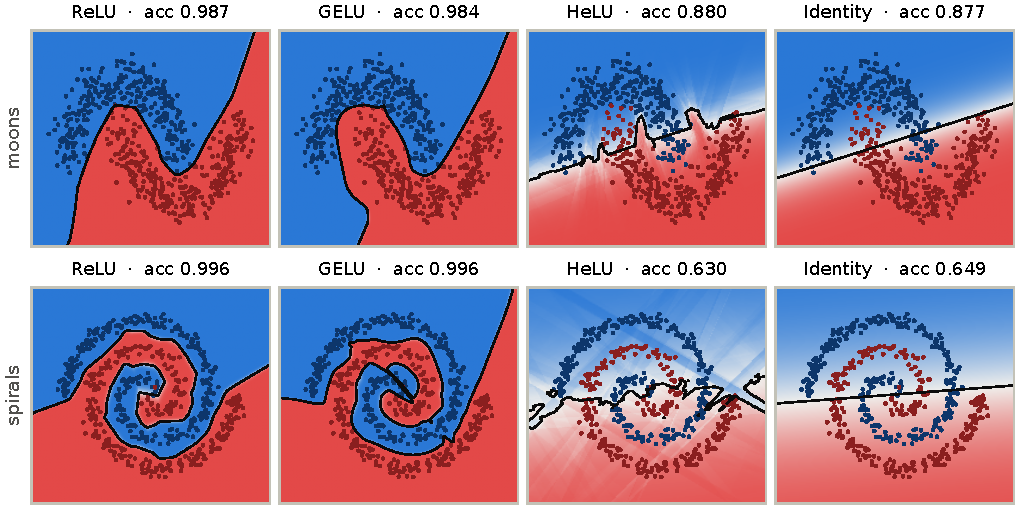
\includegraphics[width=\linewidth]{fig_cls2d.pdf}
  \caption{Decision functions on two-moons (top) and two-spirals (bottom), E3. Colour is the predicted
  probability of class 1; the black curve is the 0.5 level set. Titles give mean test accuracy over 5
  seeds. HeLU produces the linear control's straight boundary with small, spiky perturbations where
  hidden pre-activations cross the notch.}
  \label{fig:cls2d}
\end{figure}

\begin{table}[t]
  \centering\small
  \caption{2-D classification test accuracy (mean $\pm$ sd over 5 seeds) and Welch $p$-values for the
  difference between HeLU and each non-linear baseline.}
  \label{tab:cls2d}
  \begin{tabular}{lcccccc}
\toprule
 & \multicolumn{4}{c}{Test accuracy} & \multicolumn{2}{c}{$p$ (HeLU vs.)} \\
\cmidrule(lr){2-5}\cmidrule(lr){6-7}
Dataset & ReLU & GELU & HeLU & Linear & ReLU & GELU \\
\midrule
moons & 0.9873 $\pm$ 0.0017 & 0.9845 $\pm$ 0.0016 & 0.8803 $\pm$ 0.0078 & 0.8769 $\pm$ 0.0032 & $<10^{-4}$ & $<10^{-4}$ \\
spirals & 0.9962 $\pm$ 0.0016 & 0.9963 $\pm$ 0.0024 & 0.6303 $\pm$ 0.0121 & 0.6486 $\pm$ 0.0061 & $<10^{-4}$ & $<10^{-4}$ \\
\bottomrule
\end{tabular}

\end{table}

Two-moons and two-spirals are the canonical tests of whether a model can learn a curved decision
boundary. Figure~\ref{fig:cls2d} shows that ReLU and GELU do, reaching \accMoonsRelu\% and
\accMoonsGelu\% on moons and \accSpiralsRelu\% and \accSpiralsGelu\% on spirals. HeLU reaches
\accMoonsHelu\% on moons and \accSpiralsHelu\% on spirals, against \accMoonsIdentity\% and
\accSpiralsIdentity\% for the linear control (Table~\ref{tab:cls2d}). Its decision boundary is the
linear control's straight line with small, spiky perturbations where a hidden unit's pre-activation
crosses the notch, visible as faint striations in Figure~\ref{fig:cls2d}. On moons these perturbations
buy a fraction of a percentage point; on spirals they cost one, and HeLU is slightly \emph{worse} than
a linear classifier. In neither case does HeLU approach the non-linear baselines, and both differences
from ReLU and GELU are significant at $p<10^{-4}$.

\subsection{Image classification}

\begin{figure}[t]
  \centering
  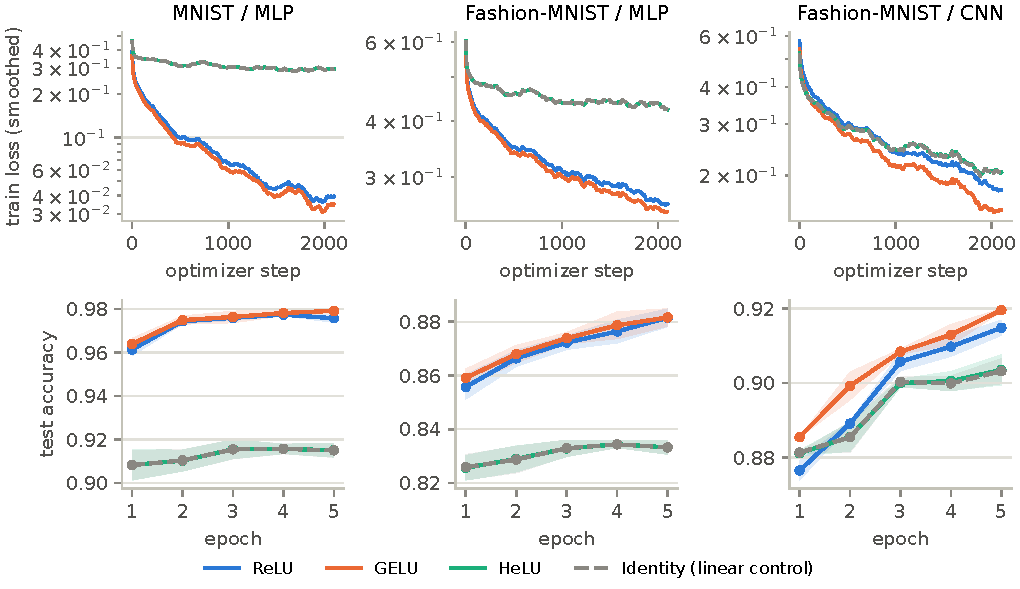
\includegraphics[width=\linewidth]{fig_curves.pdf}
  \caption{Training dynamics on the image benchmarks (E4, E5). Top: training loss, averaged over seeds
  after a 25-step moving average. Bottom: test accuracy after each epoch, shaded bands are $\pm1$ sd
  over seeds.}
  \label{fig:curves}
\end{figure}

\begin{figure}[t]
  \centering
  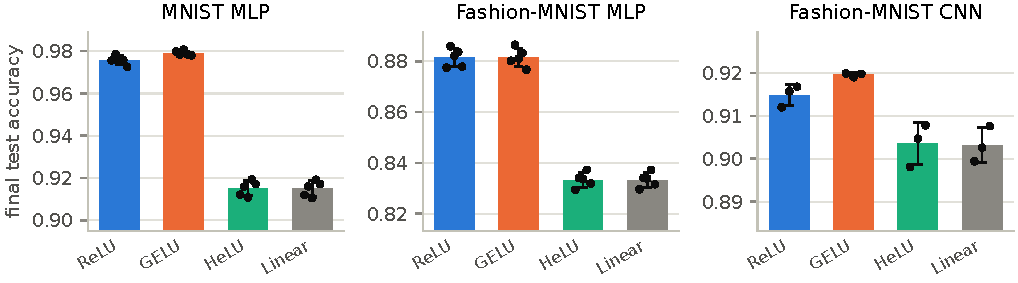
\includegraphics[width=\linewidth]{fig_summary.pdf}
  \caption{Final test accuracy on the image benchmarks. Bars are means, whiskers are $\pm1$ sd, dots
  are seeds. Note the truncated $y$-axes.}
  \label{fig:summary}
\end{figure}

\begin{table}[t]
  \centering\small
  \caption{Image benchmarks: final test accuracy (mean $\pm$ sd; 5 seeds for the MLPs, 3 for the CNN)
  and Welch $p$-values for HeLU against each other activation.}
  \label{tab:image}
  \resizebox{\linewidth}{!}{% image benchmarks: final test accuracy, mean ± sd over seeds; Welch p-values HeLU vs others
\begin{tabular}{lcccccccc}
\toprule
 & \multicolumn{4}{c}{Test accuracy (mean $\pm$ sd)} & \multicolumn{3}{c}{$p$ (HeLU vs.)} \\
\cmidrule(lr){2-5}\cmidrule(lr){6-8}
Benchmark & ReLU & GELU & HeLU & Linear & ReLU & GELU & Linear \\
\midrule
MNIST, MLP & 0.9757 $\pm$ 0.0021 & 0.9791 $\pm$ 0.0011 & 0.9150 $\pm$ 0.0035 & 0.9150 $\pm$ 0.0036 & $<10^{-4}$ & $<10^{-4}$ & 0.98 \\
Fashion-MNIST, MLP & 0.8814 $\pm$ 0.0037 & 0.8816 $\pm$ 0.0036 & 0.8333 $\pm$ 0.0029 & 0.8333 $\pm$ 0.0029 & $<10^{-4}$ & $<10^{-4}$ & 1 \\
Fashion-MNIST, CNN & 0.9148 $\pm$ 0.0025 & 0.9196 $\pm$ 0.0005 & 0.9035 $\pm$ 0.0050 & 0.9032 $\pm$ 0.0041 & 0.0395 & 0.0293 & 0.933 \\
\bottomrule
\end{tabular}
}
\end{table}

Table~\ref{tab:image} and Figures~\ref{fig:curves} and~\ref{fig:summary} report E4 and E5.
On the MNIST MLP, ReLU and GELU reach \accMnistMlpRelu\% and \accMnistMlpGelu\% while HeLU reaches
\accMnistMlpHelu\%, essentially the accuracy of a multinomial logistic regression, which is what a deep
linear network trained with cross-entropy computes (linear control: \accMnistMlpIdentity\%). On the
Fashion-MNIST MLP the gap is similar: \accFashionMlpRelu\% and \accFashionMlpGelu\% against
\accFashionMlpHelu\% (linear: \accFashionMlpIdentity\%). In both cases the HeLU-versus-ReLU and
HeLU-versus-GELU differences are significant at the $p<0.05$ level, whereas HeLU versus the linear
control is not. The training-loss curves in Figure~\ref{fig:curves} show that HeLU does not optimise
faster in early training either: its loss tracks the linear control's from the first steps and plateaus
at the same, higher, level.

The convolutional network narrows the gap without closing it. Here HeLU reaches \accFashionCnnHelu\%,
about one point below ReLU (\accFashionCnnRelu\%, $p=0.04$) and GELU (\accFashionCnnGelu\%,
$p=0.03$). But the linear control also reaches \accFashionCnnIdentity\%, and HeLU is again
indistinguishable from it ($p=0.93$). The reason the gap is small is that the architecture contains a
second non-linearity, the $2\times2$ max-pooling after each convolution. Max-pooling alone is enough to
make the convolutional network a competent non-linear classifier on this dataset, so the activation
function's contribution is largely masked. The CNN result is therefore mostly evidence about
max-pooling, not about HeLU; a network with no activation at all obtains the same accuracy.

\subsection{Depth}

\begin{figure}[t]
  \centering
  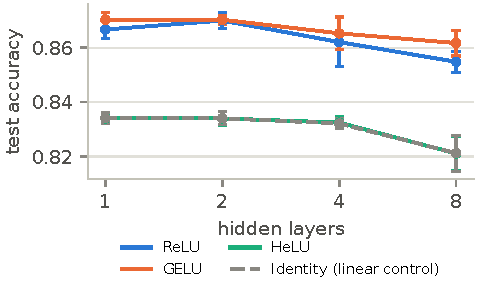
\includegraphics[width=0.5\linewidth]{fig_depth.pdf}
  \caption{Fashion-MNIST MLP test accuracy versus number of hidden layers (E6), 3 epochs, 3 seeds.}
  \label{fig:depth}
\end{figure}

\begin{table}[t]
  \centering\small
  \caption{Depth sweep on Fashion-MNIST (mean $\pm$ sd over 3 seeds).}
  \label{tab:depth}
  \begin{tabular}{lcccc}
\toprule
Hidden layers & ReLU & GELU & HeLU & Linear \\
\midrule
1 & 0.8667 $\pm$ 0.0033 & 0.8703 $\pm$ 0.0027 & 0.8340 $\pm$ 0.0017 & 0.8341 $\pm$ 0.0020 \\
2 & 0.8700 $\pm$ 0.0029 & 0.8703 $\pm$ 0.0017 & 0.8340 $\pm$ 0.0025 & 0.8341 $\pm$ 0.0024 \\
4 & 0.8621 $\pm$ 0.0089 & 0.8653 $\pm$ 0.0060 & 0.8325 $\pm$ 0.0023 & 0.8321 $\pm$ 0.0019 \\
8 & 0.8548 $\pm$ 0.0038 & 0.8617 $\pm$ 0.0048 & 0.8211 $\pm$ 0.0062 & 0.8212 $\pm$ 0.0066 \\
\bottomrule
\end{tabular}

\end{table}

If the notch were being used as a non-linearity, stacking more HeLU layers would compound it and
accuracy would change with depth in a way that differs from the linear control. Figure~\ref{fig:depth}
and Table~\ref{tab:depth} show no such divergence: HeLU's accuracy is flat from one to four hidden
layers and degrades at eight, and it coincides with the linear control to within $0.05$ percentage
points at every depth. (ReLU and GELU also degrade slightly at depth 8 under this short, untuned
3-epoch budget, but they remain $3$--$4$ points above the linear pair throughout.) A product of affine
maps is an affine map, and adding HeLU layers does not change that in practice.

\subsection{Mechanism: HeLU networks are linear}
\label{sec:mechanism}

\begin{figure}[t]
  \centering
  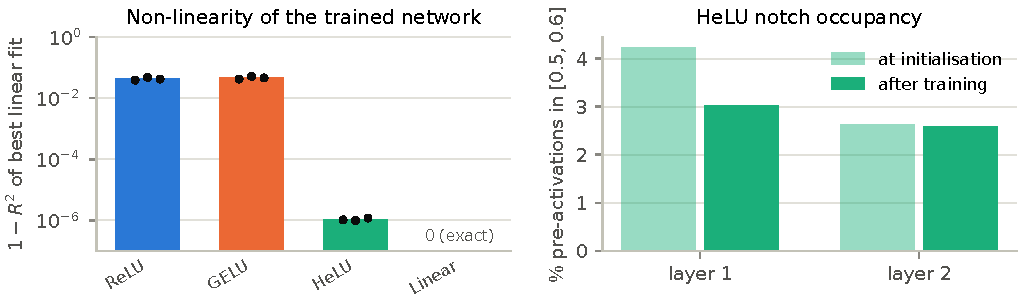
\includegraphics[width=\linewidth]{fig_linearity.pdf}
  \caption{E7. Left: $1-R^2$ of the best affine fit to each trained network's logits (log scale; lower
  means more linear). Right: percentage of HeLU pre-activations that fall inside the notch, per hidden
  layer, before and after training.}
  \label{fig:linearity}
\end{figure}

\begin{table}[t]
  \centering\small
  \caption{Linearity of trained Fashion-MNIST MLPs and notch occupancy (means over 3 seeds). The
  notch-occupancy column for ReLU, GELU, and Identity reports the fraction of \emph{their} pre-activations
  that happen to fall in $[0.5,0.6]$ and is included for reference only.}
  \label{tab:linearity}
  \begin{tabular}{lccccc}
\toprule
 & & \multicolumn{2}{c}{$R^2$ of linear fit} & \multicolumn{2}{c}{\% pre-act.\ in $[0.5,0.6]$} \\
\cmidrule(lr){3-4}\cmidrule(lr){5-6}
Activation & Test acc. & init & trained & init & trained \\
\midrule
ReLU & 0.8707 & 0.92093 & 0.95737 & 2.65 & 1.26 \\
GELU & 0.8740 & 0.95841 & 0.95385 & 2.41 & 1.35 \\
HeLU & 0.8328 & 0.99918 & 1.00000 & 3.44 & 2.81 \\
Identity (linear control) & 0.8328 & 1.00000 & 1.00000 & 3.45 & 2.80 \\
\bottomrule
\end{tabular}

\end{table}

Two direct measurements explain the results above (Figure~\ref{fig:linearity}, Table~\ref{tab:linearity}).
First, an affine function of the raw pixels explains an $R^2$ of \rTwoHelu{} of the variance in a
trained HeLU network's logits, against \rTwoRelu{} for ReLU. The HeLU network is linear to within
measurement precision. Second, only about \notchHelu\% of hidden pre-activations lie inside the notch
after training, and training does not increase this fraction relative to initialisation. Gradient
descent has no incentive to move pre-activations into the notch: doing so changes the unit's output by
at most $0.06$ and its gradient by 10\%, which is too small a lever to be worth the loss incurred on the
way. The notch is not so much unhelpful as unused.

\subsection{Computational cost}

\begin{table}[t]
  \centering\small
  \caption{Cost. Rows 1--3: median wall-clock seconds per training epoch over seeds (4 CPU threads on
  a shared machine; the median is used because a few runs overlapped with other jobs). Last row:
  forward plus backward time of the activation kernel alone, measured on an otherwise idle machine.}
  \label{tab:time}
  \begin{tabular}{lcccc}
\toprule
 & ReLU & GELU & HeLU & Linear \\
\midrule
MNIST, MLP & 1.5 & 1.6 & 1.8 & 1.5 \\
Fashion-MNIST, MLP & 1.6 & 1.6 & 1.7 & 1.4 \\
Fashion-MNIST, CNN & 12.6 & 13.5 & 17.2 & 11.7 \\
\midrule Activation kernel, fwd+bwd, 4M elements (ms) & 1.1 & 2.3 & 6.8 & 0.5 \\
\bottomrule
\end{tabular}

\end{table}

Table~\ref{tab:time} shows that HeLU is not cheaper either. Implemented as a masked \texttt{where}
with two comparisons, its forward-plus-backward kernel is about $6\times$ slower than ReLU's and
$3\times$ slower than GELU's in our PyTorch CPU measurement. End-to-end epoch time is dominated by the
linear layers, so the difference is small in practice, but there is no efficiency argument for HeLU.

\subsection{Variants of the notch}
\label{sec:variants}

\IfFileExists{generated/tab_variants.tex}{%
\begin{figure}[t]
  \centering
  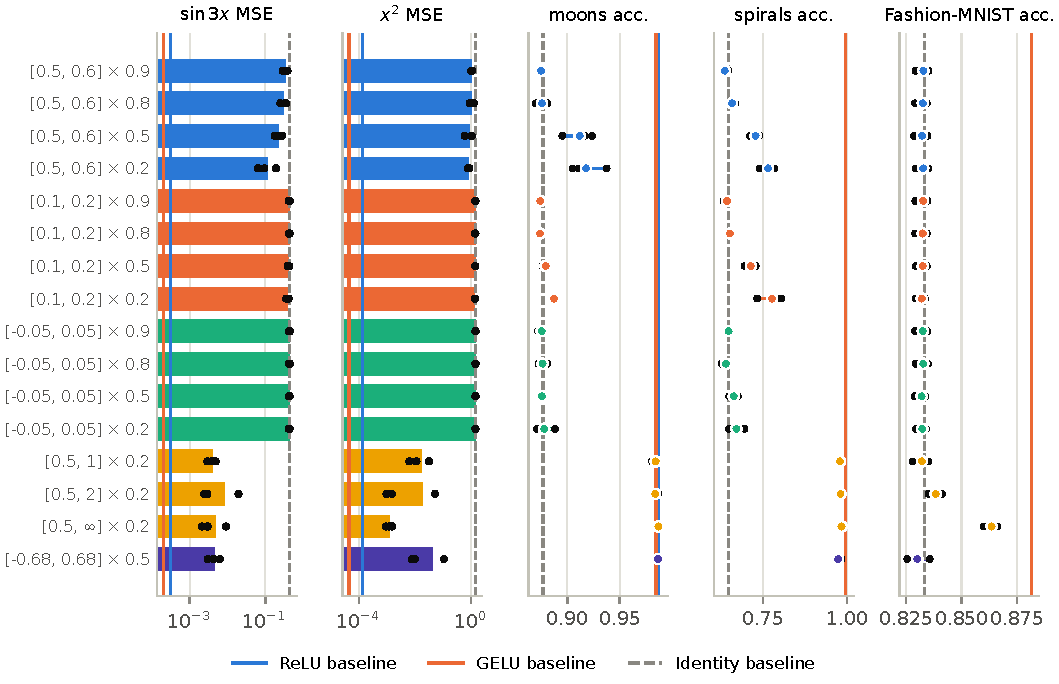
\includegraphics[width=\linewidth]{fig_variants.pdf}
  \caption{E9: sixteen variants of the HeLU notch, written as $[\text{lo},\text{hi}]\times\text{scale}$.
  The first row is the original HeLU. MSE panels (log scale): bars are means over 3 seeds. Accuracy
  panels (truncated axes): the large marker is the mean and the short line spans the seeds. Small
  black dots are individual seeds, and the vertical lines are the ReLU, GELU, and linear-control means
  from the main experiments. Colour groups variants by notch position; yellow marks the widened
  notches and violet the symmetric band $[-0.68,0.68]\times0.5$.}
  \label{fig:variants}
\end{figure}

\begin{table}[t]
  \centering\small
  \caption{E9: HeLU variants (means over 3 seeds; Fashion-MNIST also shows sd). MSE lower is better,
  accuracy higher is better. Baselines from the main experiments are repeated at the bottom.}
  \label{tab:variants}
  \resizebox{\linewidth}{!}{\begin{tabular}{llccccc}
\toprule
Notch & Scale & $\sin 3x$ MSE & $x^2$ MSE & Moons (\%) & Spirals (\%) & Fashion-MNIST (\%) \\
\midrule
$[0.5,\,0.6]$ & 0.9 & 0.342 & 1.075 & 87.5 & 63.7 & 83.29 $\pm$ 0.31 \\
$[0.5,\,0.6]$ & 0.8 & 0.310 & 1.080 & 87.6 & 65.9 & 83.26 $\pm$ 0.30 \\
$[0.5,\,0.6]$ & 0.5 & 0.221 & 0.894 & 91.2 & 72.8 & 83.23 $\pm$ 0.32 \\
$[0.5,\,0.6]$ & 0.2 & 0.117 & 0.826 & 91.8 & 76.5 & 83.28 $\pm$ 0.30 \\
$[0.1,\,0.2]$ & 0.9 & 0.433 & 1.433 & 87.4 & 64.3 & 83.27 $\pm$ 0.31 \\
$[0.1,\,0.2]$ & 0.8 & 0.431 & 1.424 & 87.4 & 65.2 & 83.26 $\pm$ 0.29 \\
$[0.1,\,0.2]$ & 0.5 & 0.408 & 1.405 & 87.9 & 71.4 & 83.26 $\pm$ 0.28 \\
$[0.1,\,0.2]$ & 0.2 & 0.382 & 1.377 & 88.7 & 77.7 & 83.21 $\pm$ 0.25 \\
$[-0.05,\,0.05]$ & 0.9 & 0.435 & 1.449 & 87.6 & 64.8 & 83.26 $\pm$ 0.30 \\
$[-0.05,\,0.05]$ & 0.8 & 0.436 & 1.449 & 87.6 & 64.0 & 83.28 $\pm$ 0.30 \\
$[-0.05,\,0.05]$ & 0.5 & 0.431 & 1.449 & 87.6 & 66.3 & 83.21 $\pm$ 0.27 \\
$[-0.05,\,0.05]$ & 0.2 & 0.431 & 1.445 & 87.8 & 67.2 & 83.24 $\pm$ 0.25 \\
$[0.5,\,1]$ & 0.2 & 0.004 & 0.016 & 98.4 & 97.9 & 83.22 $\pm$ 0.37 \\
$[0.5,\,2]$ & 0.2 & 0.008 & 0.018 & 98.4 & 98.0 & 83.84 $\pm$ 0.30 \\
$[0.5,\,\infty]$ & 0.2 & 0.005 & 0.001 & 98.7 & 98.3 & 86.36 $\pm$ 0.33 \\
$[-0.68,\,0.68]$ & 0.5 & 0.005 & 0.042 & 98.6 & 97.3 & 83.01 $\pm$ 0.51 \\
\midrule
\multicolumn{2}{l}{ReLU} & 0.0003 & 0.0001 & 98.7 & 99.6 & 88.14 \\
\multicolumn{2}{l}{GELU} & 0.0002 & 0.0000 & 98.4 & 99.6 & 88.16 \\
\multicolumn{2}{l}{Identity (linear control)} & 0.4364 & 1.4361 & 87.7 & 64.9 & 83.33 \\
\bottomrule
\end{tabular}
}
\end{table}

\begin{table}[t]
  \centering\small
  \caption{Band occupancy and linearity for the original notch, the three widened variants, and the
  symmetric band (Fashion-MNIST MLP, 3 epochs, means over 3 seeds). ``\% pre-act.\ in band'' is the
  fraction of hidden pre-activations inside $[\text{lo},\text{hi}]$, averaged over the two hidden
  layers.}
  \label{tab:variant-occupancy}
  \begin{tabular}{llcccc}
\toprule
 & & & \multicolumn{2}{c}{\% pre-act.\ in band} & \\
\cmidrule(lr){4-5}
Notch & Scale & Test acc.\ (\%) & init & trained & $R^2$ trained \\
\midrule
$[0.5,\,0.6]$ & 0.9 & 83.28 & 3.4 & 2.8 & 1.0000 \\
$[0.5,\,1]$ & 0.2 & 83.17 & 9.2 & 13.5 & 0.9992 \\
$[0.5,\,2]$ & 0.2 & 83.75 & 10.4 & 30.7 & 0.9923 \\
$[0.5,\,\infty]$ & 0.2 & 86.44 & 10.4 & 54.7 & 0.9734 \\
$[-0.68,\,0.68]$ & 0.5 & 83.01 & 87.8 & 39.6 & 0.9997 \\
\bottomrule
\end{tabular}

\end{table}

A natural objection to the results so far is that the constants in \eqref{eq:helu} are arbitrary and a
different notch might work. E9 tests this directly (Figure~\ref{fig:variants},
Table~\ref{tab:variants}). Four findings stand out.

\paragraph{Moving the notch does nothing.} Placing the notch at $[0.1,0.2]$ or straddling zero at
$[-0.05,0.05]$ gives, for every scale, results indistinguishable from the linear control on all five
tasks. The original position at $[0.5,0.6]$ is, if anything, the best of the three narrow positions,
because a small fraction of pre-activations naturally land there at initialisation.

\paragraph{Deepening the notch helps only on toy problems.} Lowering the scale from $0.9$ to $0.2$ at
$[0.5,0.6]$ reduces the $\sin 3x$ MSE from $0.34$ to $0.12$ and raises spirals accuracy from $64\%$ to
$77\%$, but ReLU and GELU are at $3\times10^{-4}$ and $99.6\%$ on the same tasks. On Fashion-MNIST none
of the twelve narrow-notch variants moves more than $0.1$ percentage points from the linear control's
$83.3\%$. A deeper notch makes each jump larger but does not make the network more inclined to use it.

\paragraph{Widening the notch changes the character of the function.} The three variants that widen the
band at scale $0.2$ behave differently from all the others. On the toy problems they close most of the
gap to ReLU: $[0.5,1.0]\times0.2$ reaches $98.4\%$ on moons and $97.9\%$ on spirals and fits $\sin 3x$
with MSE $0.004$. On Fashion-MNIST, however, the bounded bands still fail: $[0.5,1.0]$ is at the linear
level and $[0.5,2.0]$ gains only half a point. Only the unbounded variant $[0.5,\infty)\times0.2$, which
is no longer a notch at all but a two-slope piecewise-linear function with a downward jump at $0.5$,
reaches \bestVariantFashionAcc\%; that is a real non-linearity, though still $1.8$ points below ReLU.
Table~\ref{tab:variant-occupancy} shows why. After training, only $13.5\%$ of the $[0.5,1.0]$ variant's
pre-activations sit inside its band and the network is still linear to $R^2=0.9992$; the $[0.5,2.0]$
band is occupied by $31\%$ and $R^2$ drops to $0.992$; the half-line $[0.5,\infty)$ is occupied by
$55\%$ of units and $R^2$ falls to $0.973$, comparable to the $0.957$ of a ReLU network. A bounded
band, however deep, is an ``identity plus local dent'' whose effect averages out over a unit's input
distribution unless the network concentrates that distribution inside the band, and gradient descent
on a high-dimensional problem does not do so. A function that behaves differently on an entire half-line
is what forces every unit to be non-linear, and that is exactly the property that ReLU and GELU have
and HeLU lacks.

\paragraph{A wide band around zero is escaped rather than used.} The symmetric variant
$[-0.68,0.68]\times0.5$ is the strongest test of the ``too small, too rarely visited'' explanation,
because it is neither: at initialisation $78$--$98\%$ of Fashion-MNIST pre-activations lie inside it
(Table~\ref{tab:variant-occupancy}). On the toy problems it behaves like the widened notches
($98.7\%$ on moons, $97.3\%$ on spirals, $\sin 3x$ MSE $0.005$). On Fashion-MNIST it reaches
$83.0\%$, again the linear level, and after training the band occupancy has fallen to about $40\%$
while the network remains linear to $R^2=0.9997$. Both halves of this function are linear ($0.5x$
inside, $x$ outside), so a unit is non-linear only if its input distribution straddles $\pm0.68$; the
measurements are consistent with training sorting units into one regime or the other rather than
exploiting the edges. Where a bounded band ends, the function returns to the identity, and the
network can always find a linear solution by arranging for that.
}{\emph{(Variant results pending: run \texttt{python run\_all.py variants} and rebuild.)}}

\IfFileExists{generated/tab_sawtooth.tex}{%
\subsection{A sawtooth function}
\label{sec:sawtooth}

\begin{figure}[t]
  \centering
  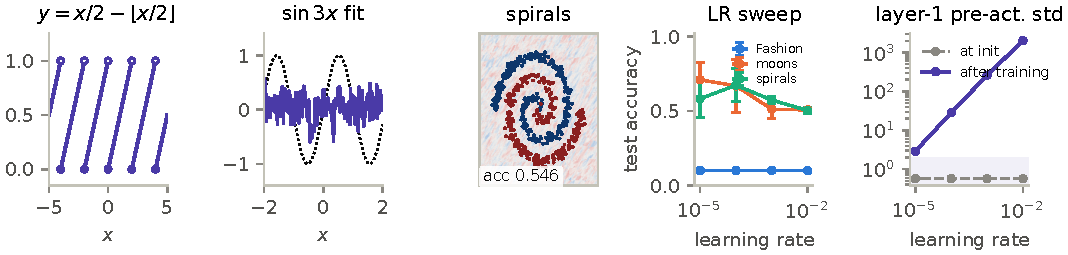
\includegraphics[width=\linewidth]{fig_sawtooth.pdf}
  \caption{E10. From left: the sawtooth $T(x)=x/2-\lfloor x/2\rfloor$ (filled and open circles mark the
  closed and open ends of each ramp); the seed-0 fit to $\sin 3x$ (target dotted); the spirals decision
  function; test accuracy versus learning rate on the three classification tasks (dotted line is chance
  on Fashion-MNIST); and the standard deviation of first-layer pre-activations on Fashion-MNIST before
  and after training (the shaded band is one period of $T$).}
  \label{fig:sawtooth}
\end{figure}

\begin{table}[t]
  \centering\small
  \caption{E10: the sawtooth against the main baselines at the default learning rates (means over 3
  seeds; Fashion-MNIST also shows sd). $R^2$ is the linear-fit coefficient of the trained Fashion-MNIST
  network.}
  \label{tab:sawtooth}
  \resizebox{\linewidth}{!}{\begin{tabular}{lcccccc}
\toprule
Activation & $\sin 3x$ MSE & $x^2$ MSE & Moons (\%) & Spirals (\%) & Fashion-MNIST (\%) & $R^2$ \\
\midrule
Sawtooth & 0.4904 & 1.4809 & 50.2 & 54.6 & 10.10 $\pm$ 0.10 & 0.3939 \\
\midrule
ReLU & 0.0003 & 0.0001 & 98.7 & 99.6 & 88.14 & 0.9574 \\
GELU & 0.0002 & 0.0000 & 98.4 & 99.6 & 88.16 & 0.9538 \\
HeLU & 0.3695 & 1.1113 & 88.0 & 63.0 & 83.33 & 1.0000 \\
Identity (linear control) & 0.4364 & 1.4361 & 87.7 & 64.9 & 83.33 & 1.0000 \\
\bottomrule
\end{tabular}
}
\end{table}

\begin{table}[t]
  \centering\small
  \caption{E10 diagnostics. Left: sawtooth learning-rate sweep (3 seeds; Fashion-MNIST after 3 epochs,
  chance is $10\%$; ``final train loss'' is the last 20 mini-batches, chance is $\ln 10\approx2.303$).
  Right: percentage of 50 initial mini-batches on which a gradient step of size $\eta$ reduced the batch
  loss.}
  \label{tab:sawtooth-diag}
  \begin{minipage}[t]{0.62\linewidth}\centering
    \resizebox{\linewidth}{!}{\begin{tabular}{lccccc}
\toprule
Learning rate & Moons (\%) & Spirals (\%) & Fashion-MNIST (\%) & Final train loss & Layer-1 pre-act.\ std \\
\midrule
$10^{-2}$ & 50.8 & 50.4 & 9.9 & 2.361 & 0.57 $\to$ 2005.5 \\
$10^{-3}$ & 51.3 & 57.4 & 10.2 & 2.311 & 0.57 $\to$ 257.3 \\
$10^{-4}$ & 67.0 & 67.4 & 10.1 & 2.306 & 0.57 $\to$ 28.0 \\
$10^{-5}$ & 71.1 & 58.3 & 10.1 & 2.309 & 0.57 $\to$ 2.9 \\
\bottomrule
\end{tabular}
}
  \end{minipage}\hfill
  \begin{minipage}[t]{0.34\linewidth}\centering
    \resizebox{\linewidth}{!}{\begin{tabular}{lccc}
\toprule
Activation & $\eta=0.001$ & $\eta=0.01$ & $\eta=0.1$ \\
\midrule
Sawtooth & 84 & 94 & 100 \\
ReLU & 100 & 100 & 100 \\
HeLU & 100 & 100 & 100 \\
Identity & 100 & 100 & 100 \\
\bottomrule
\end{tabular}
}
  \end{minipage}
\end{table}

The final function we consider is periodic: on each interval $[k,k+2)$ with $k$ an even integer,
the output is a straight line from $(k,0)$ to $(k+2,1)$, i.e.\ $T(x)=x/2-\lfloor x/2\rfloor$
(Figure~\ref{fig:sawtooth}, left). Its derivative is $1/2$ everywhere except at the even integers,
where it drops by $1$. Unlike the notch, $T$ is bounded, strongly non-linear, and non-monotone, so a
priori it is the kind of function that could give a network real expressive power.

In practice it does not train at all. At the default learning rates, the sawtooth network reaches
\accSawMoons\% on moons, \accSawSpirals\% on spirals, and \accSawFashion\% on Fashion-MNIST, which is
chance on every task, and its $\sin 3x$ MSE (\mseSawSin) is worse than the linear control's
(Table~\ref{tab:sawtooth}, Figure~\ref{fig:sawtooth}). The learning-rate sweep in
Table~\ref{tab:sawtooth-diag} rules out a simple step-size problem: on Fashion-MNIST the training loss
stays at $\ln 10$ for every learning rate from $10^{-2}$ to $10^{-5}$, and the best result on any task
is \sawBestMoons\% on moons at $\eta=\sawBestMoonsLr$, still far below the linear control.

The failure is not one of gradient \emph{direction} in the local sense. The descent test shows that at
initialisation a small gradient step reduces the batch loss on \sawDescentLow--$100\%$ of
mini-batches, against $100\%$ for ReLU, HeLU, and the identity. The gradient is locally correct; it is
globally uninformative. Because $T$ has the same slope $1/2$ at every point of every period, the
gradient with respect to a pre-activation never depends on where in the period that pre-activation
lies, so nothing in the gradient signals that a unit has wrapped around a discontinuity. The last
column of Table~\ref{tab:sawtooth-diag} shows the consequence: at $\eta=10^{-3}$ the standard
deviation of first-layer pre-activations grows from $0.6$ at initialisation to about \sawDriftDefault{}
after three epochs, spanning hundreds of periods of $T$, and the drift scales with the learning rate.
Each step is a descent step for the current mini-batch, but the weights drift monotonically through
period after period, the features seen by the next layer change chaotically from step to step, and no
consistent representation is ever formed. The one-dimensional fit in Figure~\ref{fig:sawtooth} shows
the same pathology in miniature: a dense, high-frequency oscillation rather than a curve.

The sawtooth therefore fails for a third, distinct reason. HeLU is too nearly linear for its
non-linearity to matter; the widened notches are escaped because their non-linearity is local; and
the sawtooth is expressive enough but its periodic structure decouples the gradient from the position of
each unit within a period, so gradient descent cannot navigate it. A well-behaved activation needs a
derivative that carries information about where the unit is operating, which is exactly what the
changing slopes of ReLU and GELU provide.
}{}

\IfFileExists{generated/tab_stepslope.tex}{%
\subsection{A slope-stepping function}
\label{sec:stepslope}

\begin{figure}[t]
  \centering
  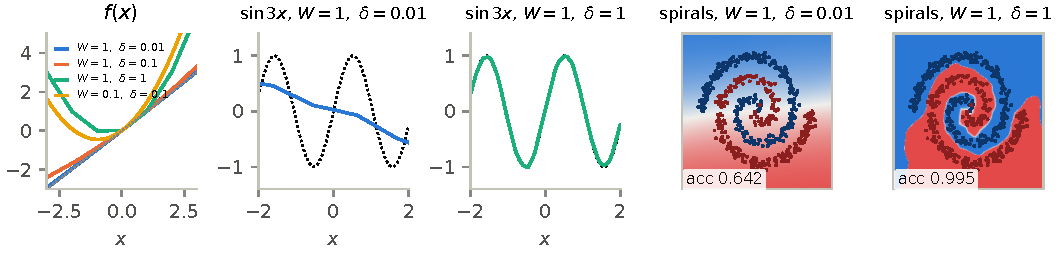
\includegraphics[width=\linewidth]{fig_stepslope.pdf}
  \caption{E11. Left: $P_{W,\delta}$ for the four settings tested (dotted line is $y=x$). Middle:
  seed-0 fits to $\sin 3x$ for the proposed setting $\delta=0.01$ and for $\delta=1$. Right: spirals
  decision functions for the same two settings, with mean test accuracy over 3 seeds.}
  \label{fig:stepslope}
\end{figure}

\begin{table}[t]
  \centering\small
  \caption{E11: the slope-stepping function against the main baselines (means over 3 seeds;
  Fashion-MNIST also shows sd). $R^2$ is the linear-fit coefficient of the trained Fashion-MNIST
  network.}
  \label{tab:stepslope}
  \resizebox{\linewidth}{!}{\begin{tabular}{llcccccc}
\toprule
$W$ & $\delta$ & $\sin 3x$ MSE & $x^2$ MSE & Moons (\%) & Spirals (\%) & Fashion-MNIST (\%) & $R^2$ \\
\midrule
1 & 0.01 & 0.4032 & 0.0001 & 88.9 & 64.2 & 82.60 $\pm$ 1.19 & 1.0000 \\
1 & 0.1 & 0.0078 & 0.0000 & 98.9 & 92.2 & 84.62 $\pm$ 0.55 & 0.9770 \\
1 & 1 & 0.0006 & 0.0001 & 98.7 & 99.5 & 86.16 $\pm$ 0.68 & 0.9120 \\
0.1 & 0.1 & 0.3053 & 0.0000 & 98.4 & 86.4 & 86.63 $\pm$ 0.51 & 0.9192 \\
\midrule
\multicolumn{2}{l}{ReLU} & 0.0003 & 0.0001 & 98.7 & 99.6 & 88.14 & 0.9574 \\
\multicolumn{2}{l}{GELU} & 0.0002 & 0.0000 & 98.4 & 99.6 & 88.16 & 0.9538 \\
\multicolumn{2}{l}{HeLU} & 0.3695 & 1.1113 & 88.0 & 63.0 & 83.33 & 1.0000 \\
\multicolumn{2}{l}{Identity (linear control)} & 0.4364 & 1.4361 & 87.7 & 64.9 & 83.33 & 1.0000 \\
\bottomrule
\end{tabular}
}
\end{table}

The last function repairs the sawtooth's two defects in turn: it is made continuous by stacking the
segments end to end, and made non-linear by letting the slope of each successive segment grow by a
fixed increment $\delta$. On segment $k=\lfloor x/W\rfloor$ the slope is $1+\delta k$, for every
integer $k$, so the function is convex, has slope exactly $1$ on $[0,W)$, and is a piecewise-linear
approximation of the parabola $x+\delta x^2/(2W)$ with a kink at every multiple of $W$
(Figure~\ref{fig:stepslope}, left). The proposal is to keep $\delta$ small, $0.01$, on the argument
that pre-activations are roughly Gaussian and rarely reach the outer segments where the slope becomes
large.

That argument is correct, and it is exactly why the proposed setting does not work. With
$\delta=0.01$ and $W=1$, the slope over the range $[-3,3]$ that contains almost all pre-activations
varies only between $0.97$ and $1.03$, and the function deviates from the identity by at most
$\delta x^2/(2W)\approx0.05$. This is the HeLU situation again: a non-linearity too small for gradient
descent to exploit. Table~\ref{tab:stepslope} confirms it. At $\delta=0.01$ the trained Fashion-MNIST
network is linear to $R^2=\rTwoSsSmall$, and every task lands at the linear control's level:
\accSsSmallFashion\% on Fashion-MNIST, \accSsSmallMoons\% on moons, \accSsSmallSpirals\% on spirals,
and a $\sin 3x$ MSE of \mseSsSmallSin. (The $x^2$ column is an exception for every setting and should
be discounted: the activation is itself nearly quadratic, so a quadratic target is trivially
representable.)

Raising the curvature turns the function into a working activation. At $\delta=0.1$ the network is no
longer linear ($R^2=\rTwoSsMid$), moons and spirals jump to \accSsMidMoons\% and \accSsMidSpirals\%,
and Fashion-MNIST gains a point over the linear control. At $\delta=1$, where the slope changes by a
full unit at each kink, the function reaches \accSsOneSpirals\% on spirals, fits $\sin 3x$ with MSE
$\mseSsOneSin$ (Figure~\ref{fig:stepslope}, middle and right), and reaches \accSsOneFashion\% on
Fashion-MNIST: a genuine non-linearity, though still two points below ReLU and GELU, which is
consistent with what is known about quadratic-like activations in small networks. The comparison
between $(W,\delta)=(1,1)$ and $(0.1,0.1)$ is instructive: both approximate the same parabola
$x+x^2/2$, but the finer segmentation reaches a similar Fashion-MNIST accuracy (\accSsFineFashion\%)
while fitting $\sin 3x$ far worse (MSE \mseSsFineSin) and losing thirteen points on spirals. The coarse
version has a sharp ReLU-like kink every unit that a small network can place and use; the fine
version is effectively a smooth parabola, and a two-hidden-layer network of parabolas is a
low-degree polynomial that cannot bend around a spiral.

The lesson of this final function is the mirror image of the sawtooth's. There, the function was
expressive but its gradient uninformative; here, the gradient is informative but the proposed
constants remove the expressiveness. The property that makes the design work when $\delta$ is large
is that the slope, and therefore the gradient, changes appreciably with the unit's operating point,
which is the same property that makes ReLU and GELU work. Choosing $\delta$ to keep the slope nearly
constant across the Gaussian bulk of the pre-activations, which the proposal does to avoid exploding
gradients, also keeps the network linear across that bulk. There is no setting of $\delta$ that is
both safe by that criterion and useful.
}{}

\IfFileExists{generated/tab_stepslope_final.tex}{%
\subsection{Tuning the slope-stepping function against GELU}
\label{sec:stepslope-tune}

\begin{figure}[t]
  \centering
  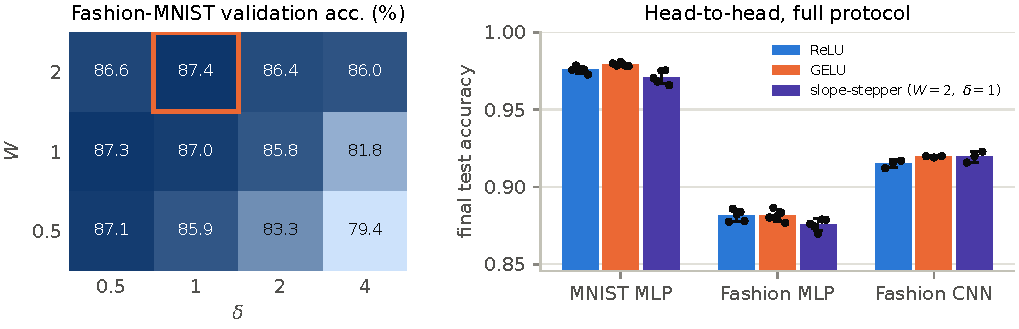
\includegraphics[width=\linewidth]{fig_stepslope_tune.pdf}
  \caption{E12. Left: mean Fashion-MNIST validation accuracy over the $(W,\delta)$ grid (3 epochs,
  3 seeds); the orange box marks the selected setting. Right: head-to-head final test accuracy of the
  selected setting against ReLU and GELU under the full protocol. Bars are means, whiskers $\pm1$ sd,
  dots are seeds.}
  \label{fig:stepslope-tune}
\end{figure}

\begin{table}[t]
  \centering\small
  \caption{E12 tuning grid. Validation accuracy on the held-out 10k split of the Fashion-MNIST training
  set after 3 epochs (mean $\pm$ sd over 3 seeds), final training loss, and toy-task results. The
  selected setting is starred. ReLU and GELU rows use the same protocol.}
  \label{tab:stepslope-tune}
  \resizebox{\linewidth}{!}{\begin{tabular}{llccccc}
\toprule
$W$ & $\delta$ & Fashion val.\ acc.\ (\%) & Train loss & $\sin 3x$ MSE & Moons (\%) & Spirals (\%) \\
\midrule
0.5 & 0.5 & 87.10 $\pm$ 0.50 & 0.343 & 0.0030 & 98.5 & 99.6 \\
0.5 & 1 & 85.88 $\pm$ 0.62 & 1.149 & 0.0007 & 98.7 & 99.6 \\
0.5 & 2 & 83.31 $\pm$ 2.76 & 0.597 & 0.0005 & 98.6 & 99.7 \\
0.5 & 4 & 79.41 $\pm$ 4.12 & 158.736 & 0.0063 & 98.6 & 99.7 \\
1 & 0.5 & 87.32 $\pm$ 0.30 & 0.314 & 0.0004 & 98.8 & 99.5 \\
1 & 1 & 87.04 $\pm$ 0.57 & 0.339 & 0.0006 & 98.7 & 99.5 \\
1 & 2 & 85.85 $\pm$ 0.78 & 0.391 & 0.0006 & 98.7 & 99.7 \\
1 & 4 & 81.81 $\pm$ 3.15 & 0.452 & 0.0023 & 98.5 & 99.6 \\
2 & 0.5 & 86.64 $\pm$ 0.66 & 0.326 & 0.0004 & 98.8 & 99.5 \\
2 & 1$^\ast$ & 87.41 $\pm$ 0.52 & 0.318 & 0.0003 & 98.4 & 99.5 \\
2 & 2 & 86.38 $\pm$ 0.35 & 0.359 & 0.0007 & 98.6 & 99.6 \\
2 & 4 & 86.02 $\pm$ 0.15 & 0.539 & 0.0008 & 98.7 & 99.6 \\
\midrule
\multicolumn{2}{l}{GELU} & 87.28 $\pm$ 1.24 & 0.301 & 0.0003 & 98.5 & 99.6 \\
\multicolumn{2}{l}{ReLU} & 86.97 $\pm$ 0.97 & 0.308 & 0.0002 & 98.8 & 99.6 \\
\bottomrule
\end{tabular}
}
\end{table}

\begin{table}[t]
  \centering\small
  \caption{E12 head-to-head: the tuned slope-stepping function against ReLU and GELU under the main
  protocols (5 seeds for the MLPs, 3 for the CNN and the depth rows), with Welch $p$-values.}
  \label{tab:stepslope-final}
  \resizebox{\linewidth}{!}{\begin{tabular}{lccccc}
\toprule
 & \multicolumn{3}{c}{Test accuracy (mean $\pm$ sd)} & \multicolumn{2}{c}{$p$ (stepper vs.)} \\
\cmidrule(lr){2-4}\cmidrule(lr){5-6}
Benchmark & ReLU & GELU & Slope-stepper & ReLU & GELU \\
\midrule
MNIST, MLP & 0.9757 $\pm$ 0.0021 & 0.9791 $\pm$ 0.0011 & 0.9709 $\pm$ 0.0042 & 0.067 & 0.0107 \\
Fashion-MNIST, MLP & 0.8814 $\pm$ 0.0037 & 0.8816 $\pm$ 0.0036 & 0.8756 $\pm$ 0.0039 & 0.0392 & 0.0359 \\
Fashion-MNIST, CNN & 0.9148 $\pm$ 0.0025 & 0.9196 $\pm$ 0.0005 & 0.9195 $\pm$ 0.0036 & 0.146 & 0.977 \\
Fashion-MNIST, MLP depth 1 (3 ep.) & 0.8667 $\pm$ 0.0033 & 0.8703 $\pm$ 0.0027 & 0.8667 $\pm$ 0.0016 & 1 & 0.134 \\
Fashion-MNIST, MLP depth 2 (3 ep.) & 0.8700 $\pm$ 0.0029 & 0.8703 $\pm$ 0.0017 & 0.8720 $\pm$ 0.0017 & 0.371 & 0.28 \\
Fashion-MNIST, MLP depth 4 (3 ep.) & 0.8621 $\pm$ 0.0089 & 0.8653 $\pm$ 0.0060 & 0.7888 $\pm$ 0.1240 & 0.414 & 0.397 \\
Fashion-MNIST, MLP depth 8 (3 ep.) & 0.8548 $\pm$ 0.0038 & 0.8617 $\pm$ 0.0048 & 0.1321 $\pm$ 0.0557 & 0.00189 & 0.00181 \\
\bottomrule
\end{tabular}
}
\end{table}

Section~\ref{sec:stepslope} showed that the slope-stepping function needs curvature of order one to
work. E12 asks whether, with its two constants tuned, it can match GELU. To keep the comparison honest
the tuning uses a validation split of the training set, the test sets are touched only once for the
head-to-head, and GELU and ReLU are run under the identical validation protocol so that the
comparison is not between a tuned function and untuned baselines on different data.

\paragraph{Tuning.} Figure~\ref{fig:stepslope-tune} (left) and Table~\ref{tab:stepslope-tune} show
the grid. The landscape is simple: validation accuracy is best along the diagonal $\delta/W\approx0.5$
to $1$ and falls off on either side. Too little curvature ($\delta/W=0.25$) leaves accuracy a point
lower; too much ($\delta/W\ge2$) makes training unstable, with rising training loss and seed variance
of several points, and at $(W,\delta)=(0.5,4)$ the loss diverges outright. The selected setting is
$W=\ssBestW$, $\delta=\ssBestDelta$, with \ssBestVal\% validation accuracy against \geluVal\% for GELU
and \reluVal\% for ReLU under the same protocol. On the toy problems every grid point is already at
the ReLU/GELU level, so the toys do not discriminate here.

\paragraph{Head-to-head.} Table~\ref{tab:stepslope-final} and Figure~\ref{fig:stepslope-tune} (right)
give the result under the full protocol. The tuned slope-stepper is a competitive activation in
shallow networks and an unusable one in deep networks.
\begin{itemize}[nosep]
  \item On the Fashion-MNIST CNN it ties GELU exactly (\finalCnnSs\% versus \finalCnnGelu\%,
        $p=\finalCnnPGelu$) and is ahead of ReLU (\finalCnnRelu\%).
  \item On the MLPs it is slightly but consistently behind: \finalMnistSs\% versus \finalMnistGelu\%
        on MNIST ($p=\finalMnistPGelu$) and \finalFashionSs\% versus \finalFashionGelu\% on
        Fashion-MNIST ($p=\finalFashionPGelu$). The gaps are under one point but significant at the
        $0.05$ level with five seeds, and the slope-stepper's seed variance is the largest of the three.
  \item In the depth sweep it is level with the baselines at one and two hidden layers
        (\depthSsTwo\% versus \depthGeluTwo\% for GELU at depth 2, $p=0.28$), degrades sharply and erratically at four
        (\depthSsFour\% with a seed spread of twelve points), and collapses to chance at eight
        (\depthSsEight\%), where GELU still reaches \depthGeluEight\%.
\end{itemize}

\paragraph{Why it breaks with depth.} The function is convex and unbounded with a slope that grows
without limit: on segment $k$ the slope is $1+k$ for the selected setting. A layer's outputs are
therefore larger and more spread out than its inputs whenever the inputs reach the outer segments,
and the next layer sees pre-activations that reach them more often still. GELU, ReLU, and every
activation in common use have slope bounded by a constant near $1$, which is what keeps signal scale
stable through depth. The slope-stepper has no such bound, and with four or more layers the
forward pass amplifies until training fails. Bounding the slope (capping $k$, or applying the stepping
only on one side) would be the natural fix, but it would also move the function toward the
piecewise-linear convex shapes that already exist in the literature.

\paragraph{Cost.} The selected setting is also slower: with a floor and several multiplies per
element, the CNN epoch takes about $2.4\times$ as long as with GELU in our PyTorch CPU
implementation (per-run wall times are in the raw results).

\paragraph{Verdict.} With $(W,\delta)=(2,1)$ the slope-stepping function is the first design in this
study that is a genuine alternative to GELU on some benchmarks: it ties GELU on the CNN and comes
within a point on the MLPs. It does not beat GELU anywhere, it is significantly behind on both MLP
benchmarks, and its unbounded slope makes it fail at depths where GELU is unaffected. Against the
original hypothesis of superiority, the tuned result is ``competitive in shallow networks, worse
overall''.
}{}

\section{Discussion}

\paragraph{Why HeLU fails.} A useful activation function must do two things: give the network a
non-linear family of functions to search over, and make that family reachable by gradient descent.
HeLU does the first only in the technical sense of \citet{leshno1993multilayer}, and the second not at
all. Its total non-linear content, a $10\%$ dip on a band of width $0.1$, is an order of magnitude
smaller than the scale of typical pre-activations at initialisation~\citep{he2015delving}, and gradient
descent finds nothing to gain by concentrating pre-activations there. The result is a network that is,
for all practical purposes, linear, and it performs exactly as a linear network does: adequately on
MNIST, where a linear classifier already reaches about $91.5\%$, and poorly everywhere a curved
boundary is required. The one place we saw the notch being used at all, the one-dimensional regression
tasks with full-batch training, it produced a jagged staircase of jumps rather than a useful curve.

\paragraph{The CNN caveat.} The Fashion-MNIST CNN result deserves emphasis because it is the kind of
evidence that could be mistaken for support. HeLU comes within about a point of ReLU on this benchmark
only because max-pooling makes the activation function nearly irrelevant, and the identity control
demonstrates this by landing at the same accuracy. Any evaluation of a new activation should include a
no-activation control for this reason.

\paragraph{What would change the conclusion.} Section~\ref{sec:variants} already answers the obvious
follow-ups. Moving the notch does nothing; deepening it helps only on one- and two-dimensional toy
problems; and the only modification that produces a non-linear network on Fashion-MNIST is to extend
the band to the whole half-line $[0.5,\infty)$, at which point the function is a two-slope piecewise
linear map with a jump, not a notch, and it still trails ReLU by about two points. We did not tune
learning rates per activation; given that HeLU's training curves coincide with the linear control's
from the first steps, we do not expect tuning to change the ordering.

\paragraph{Limitations.} All experiments are small-scale and CPU-bound: two image datasets of
$28\times28$ greyscale images, networks of at most a few hundred thousand parameters, at most 5 epochs,
and 3 to 5 seeds per configuration. The CIFAR-10 download was blocked in our environment. Larger-scale
experiments could in principle behave differently, but the mechanism identified in
Section~\ref{sec:mechanism} does not depend on scale: pre-activations avoid the notch because the
gradient signal for entering it is negligible, and that is a property of the function, not of the
dataset.

\section{Conclusion}

We set out to verify that HeLU, the identity function with a $0.9\times$ notch on $[0.5,0.6]$, is a
superior activation to ReLU and GELU. Under matched conditions across regression, two-dimensional
classification, MNIST, and Fashion-MNIST, it is not. HeLU networks are statistically indistinguishable
from purely linear networks and significantly worse than ReLU and GELU networks on every task that
requires a non-linear solution. The mechanism is simple: the notch is too small and too rarely visited to
function as a non-linearity, so the network stays linear. The only benchmark on which HeLU comes close
to the baselines is one in which max-pooling supplies the non-linearity, and a network with no
activation at all comes equally close there. An ablation over sixteen variants confirms that the
problem is the notch design rather than its constants: no bounded notch, at any position or depth we
tried, produces a non-linear network on Fashion-MNIST, and the one variant that does is no longer a
notch. A sawtooth function $x/2-\lfloor x/2\rfloor$, tested as a further alternative, stays at chance
on every classification task at every learning rate we tried, because its constant slope gives the
gradient no information about which period each unit is operating in. A continuous slope-stepping
function $x+\delta x^2/(2W)$ (piecewise-linear) trains well once $\delta$ is of order one, and with
$(W,\delta)$ tuned on a validation split it ties GELU on the Fashion-MNIST CNN and trails it by under
a point on the MLPs, the closest any design here comes; but at the proposed $\delta=0.01$ it is
indistinguishable from the linear control, and its unbounded slope makes it collapse at depth 8 where
GELU is unaffected. Across all of these designs the same rule holds: an
activation helps only if its slope changes appreciably over the range its inputs actually occupy, and
the gradient reports that change.

\section*{Reproducibility}

The code, raw JSON results for every run, figures, and this document are in the repository directory
\path{helu-activation-research/}. Running \texttt{run\_all.py} regenerates the results (about
40 minutes on four CPU cores for the main experiments, plus about 30 minutes for the variants),
\texttt{make\_figures.py} regenerates every figure and table in this paper from them, and
\texttt{make} in the \texttt{paper/} directory rebuilds the PDF.

\bibliographystyle{plainnat}
\bibliography{refs}

\end{document}
